% !TEX root = BioInspired.tex

\chapter{Fractals - Text Chapter 7}



\section{Problem 7.10}


\subsection{Problem Information}

	Write a python program to use turtle graphics to draw the fractals in figure 7.24.  This incorporates the bracketed OL-system described in chapter 7 to draw fractals.  After recreating the fractals from the book, I came up with my own set of production rules to draw even more fractals.  Unfortunately the ones I came up with were not as cool as the ones in the book.

\subsection{Implementation}

	I wrote this program in python and used the turtle graphics module to do the fractal drawing.  The functions I wrote for this program were the generate production rules function, and the draw fractal function.  To generate the production rules I simply iterated through the initial string and replaced everything corresponding to the F-rule and G-rule.  I generated the entire production rules string before I drew the fractal.  Then to draw the fractal I passed in the production rules string as well as the rotate value and the draw length.

\subsection{Issues}

	When tasked with coming up with my own production rules, most of the ones I came up with turned out to look like tumbleweeds.  I don't know why most of them did that, but some others that I produced were very stick like.  It wasn't a problem with my program, just my own lack of creativity.
	
\subsection{Analysis}

	The code to produce the fractal rules and to draw the fractal were very simple and didn't require too much work.  I made functions to call each of the different fractals with each of their own rule sets.  The fractals themselves were fun to watch for a while but ultimately they took way too long to draw so I ended up getting bored and doing something else while they were drawing. 


\begin{figure}[tbh]
\begin{center}
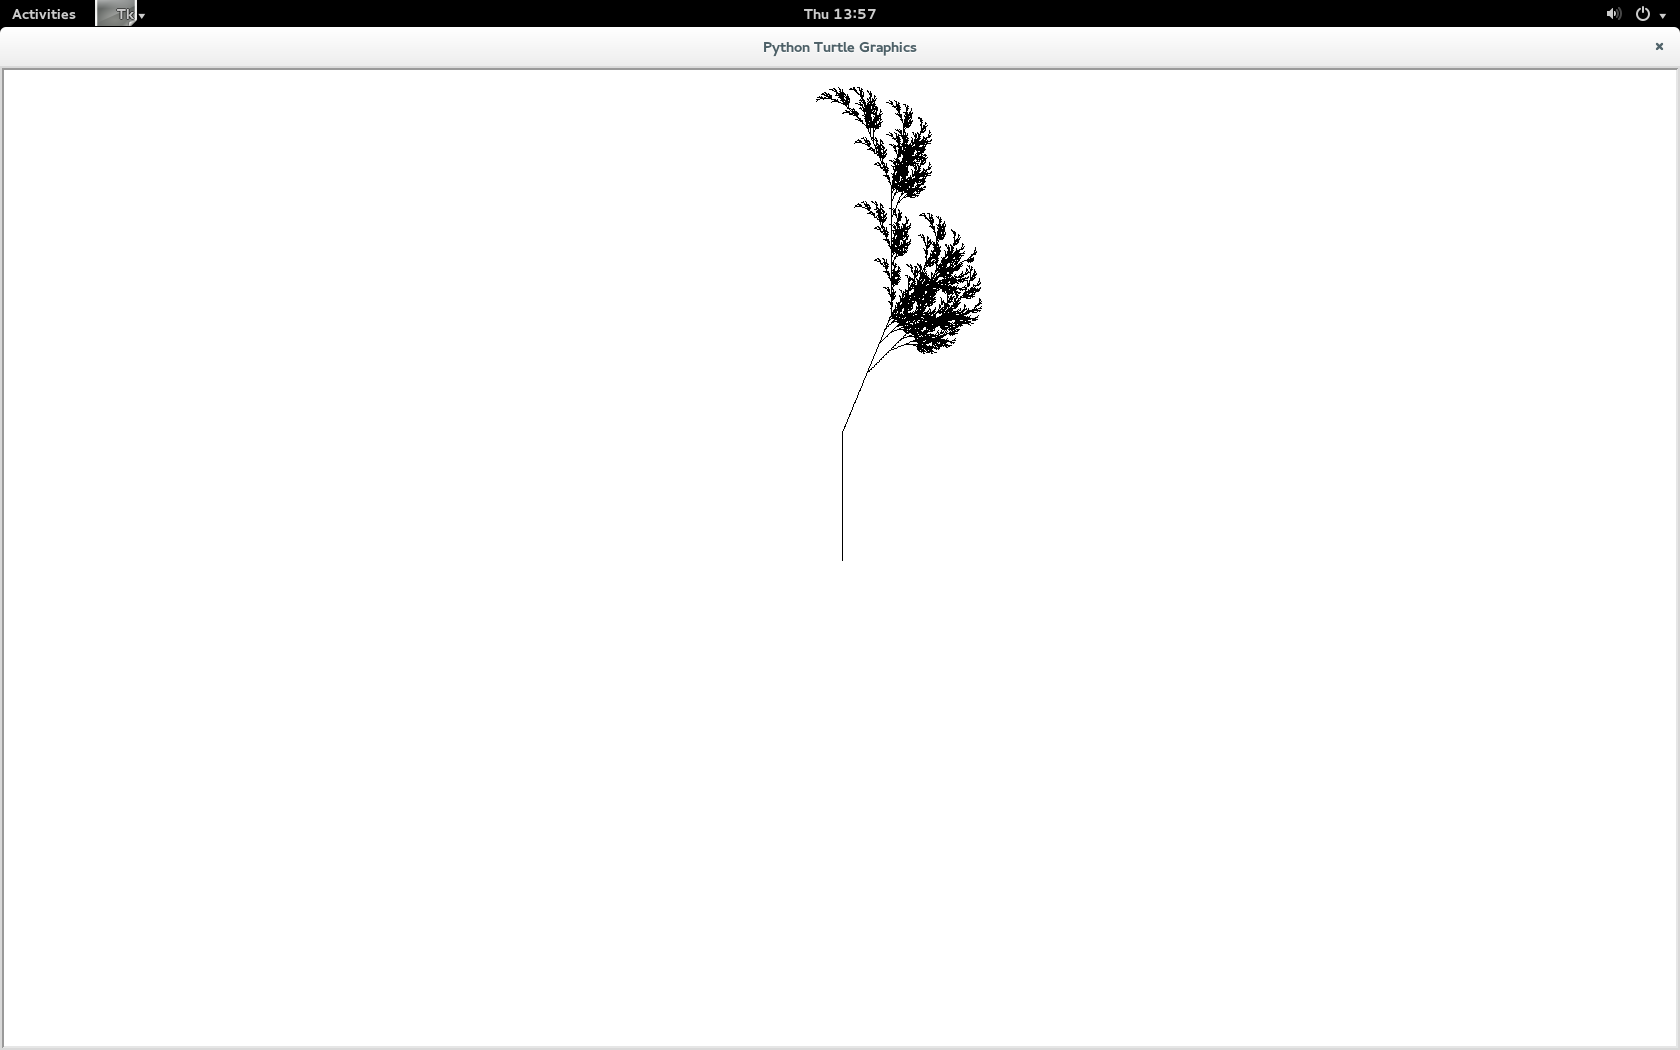
\includegraphics[width=0.75\textwidth]{fractal1.png}
\end{center}
\caption{Fractal 1\label{fig:gprun}}
\end{figure}

\begin{figure}[tbh]
\begin{center}
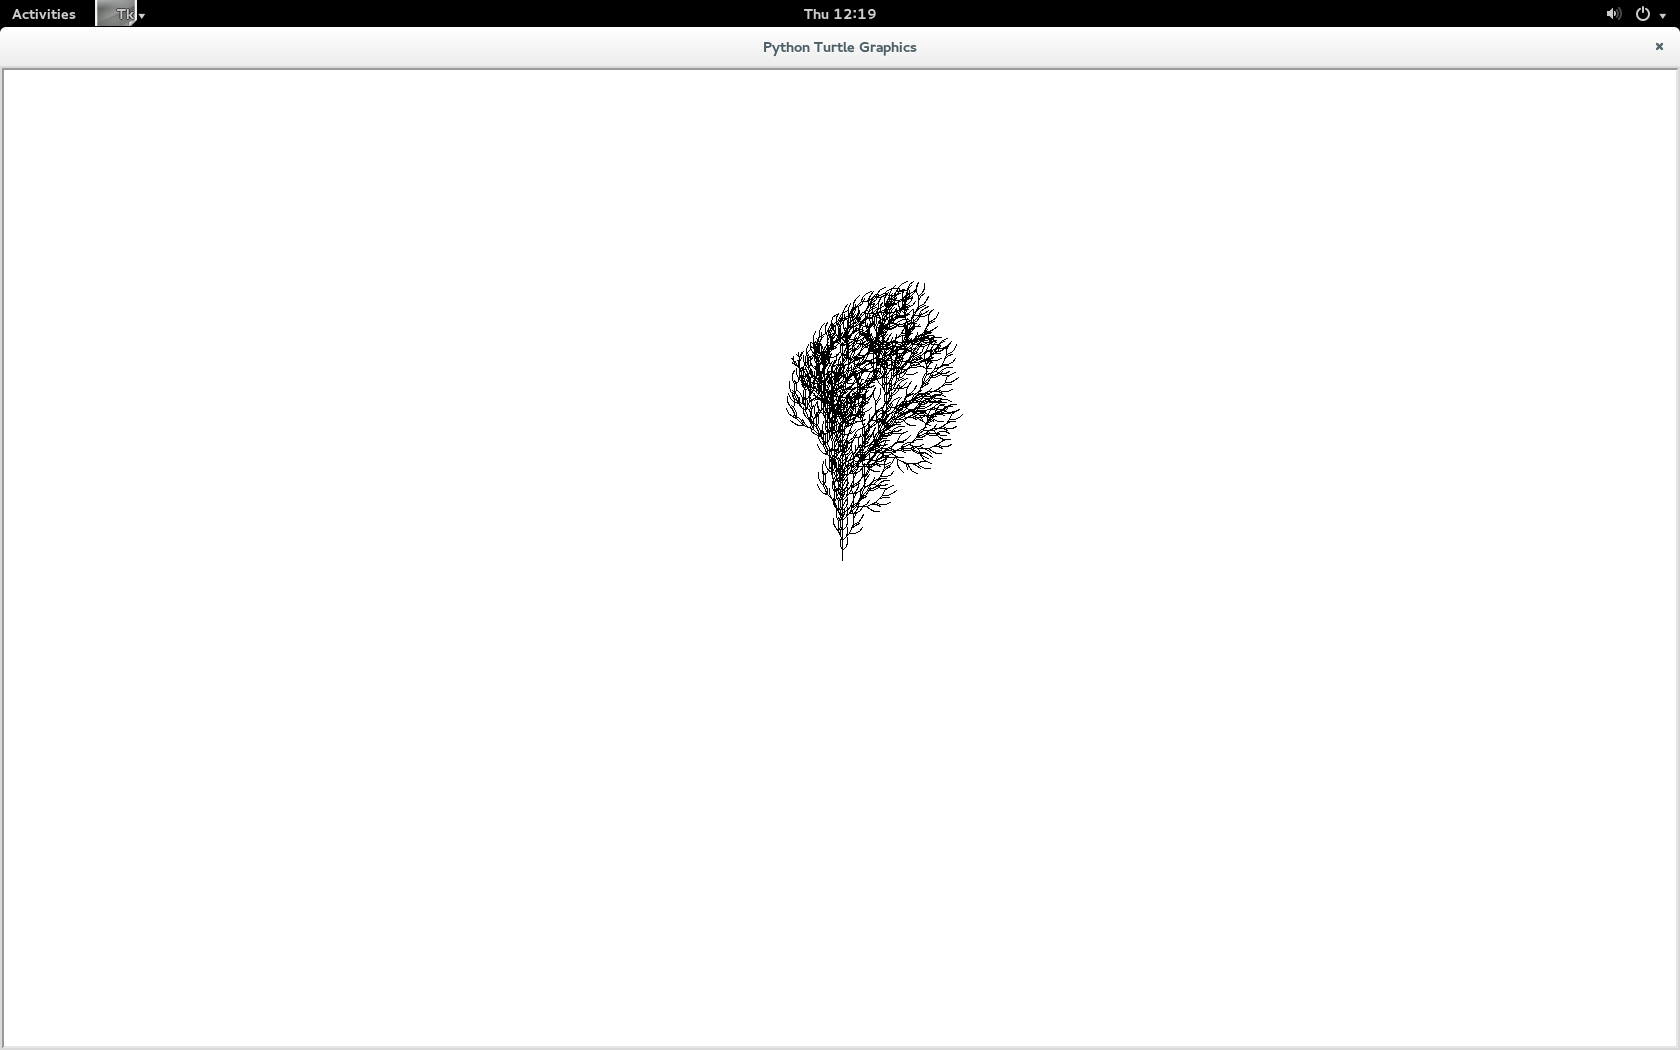
\includegraphics[width=0.75\textwidth]{fractal2.png}
\end{center}
\caption{Fractal 2\label{fig:gprun}}
\end{figure}

\begin{figure}[tbh]
\begin{center}
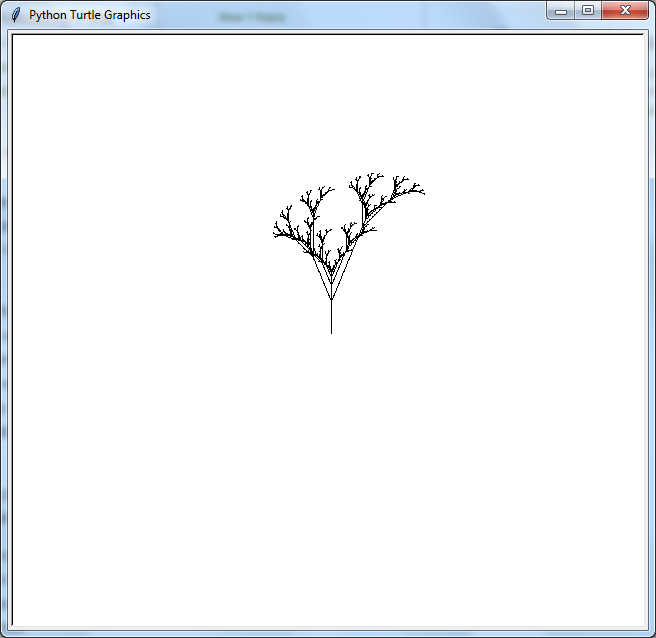
\includegraphics[width=0.75\textwidth]{fractal3.png}
\end{center}
\caption{Fractal 3\label{fig:gprun}}
\end{figure}

\begin{figure}[tbh]
\begin{center}
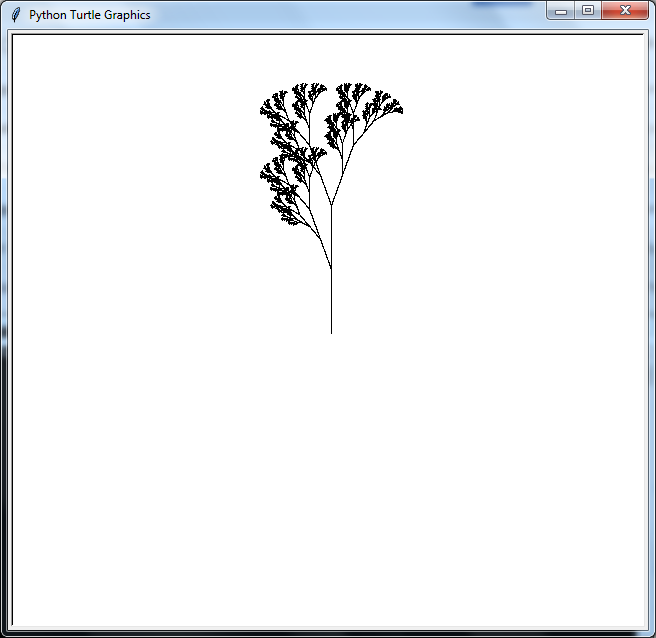
\includegraphics[width=0.75\textwidth]{fractal4.png}
\end{center}
\caption{Fractal 4\label{fig:gprun}}
\end{figure}	

\begin{figure}[tbh]
\begin{center}
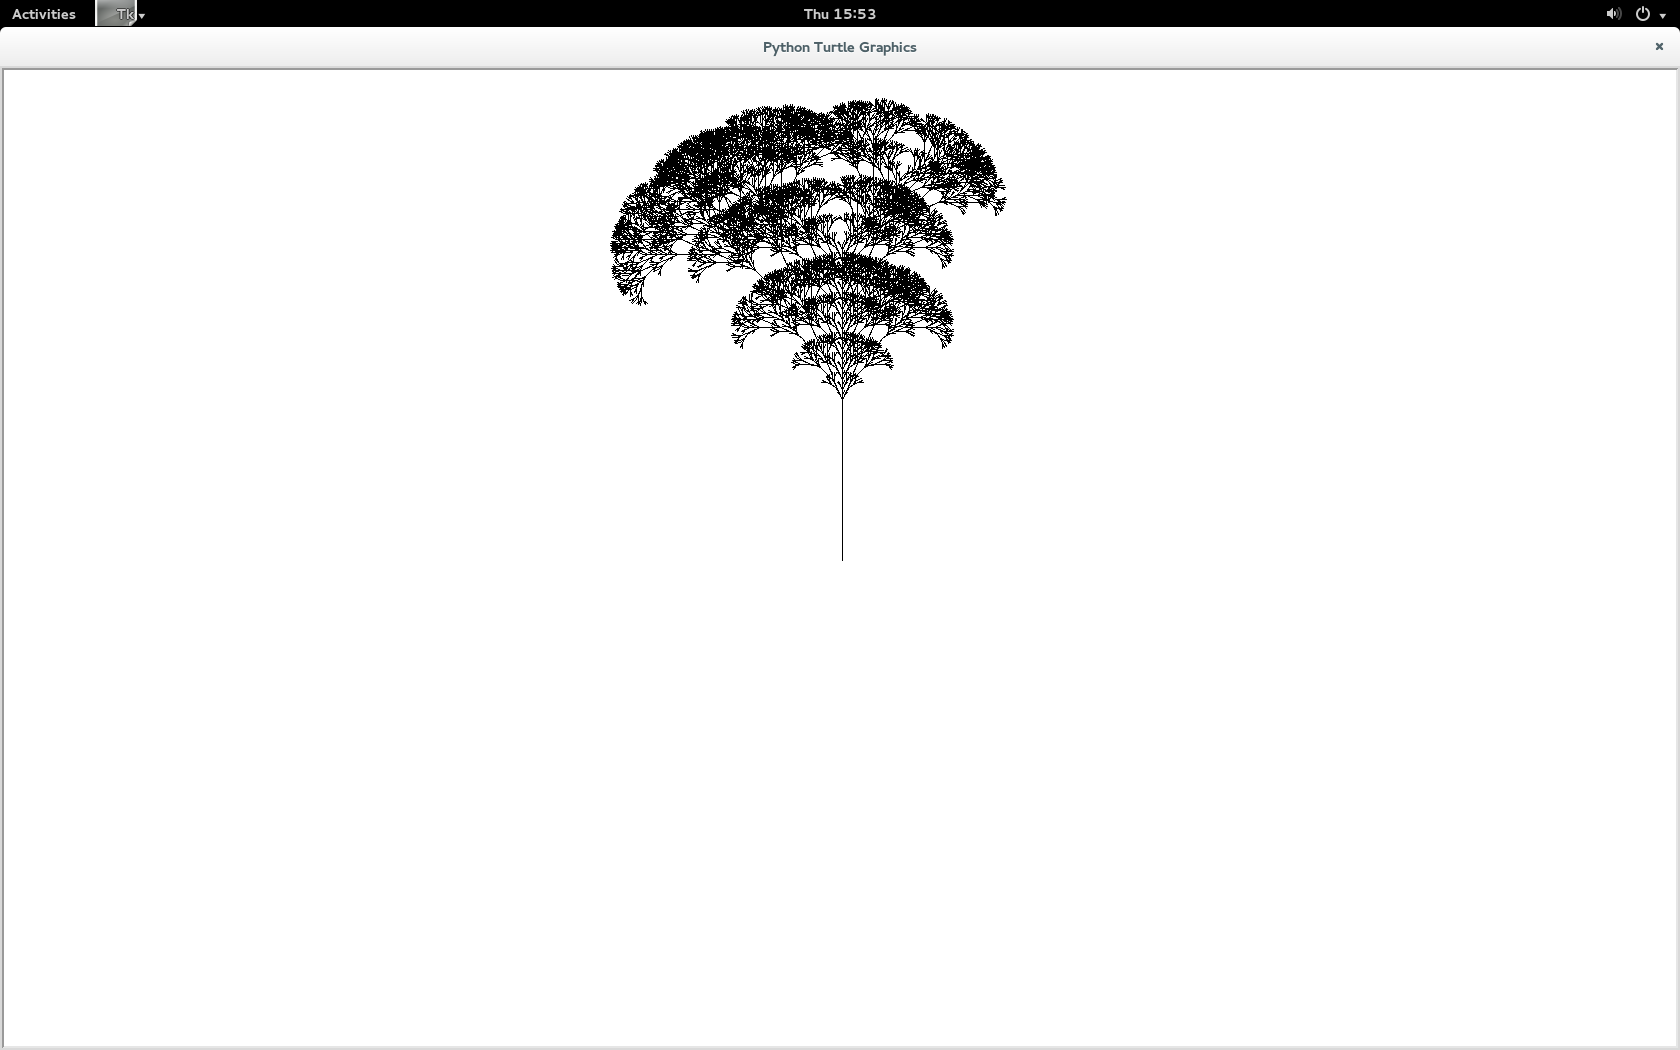
\includegraphics[width=0.75\textwidth]{fractal6.png}
\end{center}
\caption{Fractal 6\label{fig:gprun}}
\end{figure}
	


\section{Problem 7.15}

Implement a RIFS to generate all the fractals whose codes are presented in Table 7.3

\subsection{Problem Information}

RIFS - Random Iterated Function Systems - are a method of sequentially drawing fractals which give varying results.  Each iteration has a certain chance of making an affine transform on the current pixel and then updating the pixel to that transformed one.

Although RIFS systems are quite small code-wise, they can generate some very interesting shapes through emergent behaviour.  Table 7.3 presented us with some classic fractals: The Serpinski Gasket, the Bernoulli Fern, The Square and The Tree.  There was an error in the gasket's d column values - they should all be .5.

One major difference between the RIFS and IFS fractal generation systems is that while the IFS uses subimages or drawing strokes, the RIFS just uses individual pixel values.  This makes the turtle a poor fit for output, and so instead we used pyplot's scatter graph.  The results were simply lovely.

\subsection{Algorithm Description}

The RIFS algorithm we implemented came straight out of the book.  The only real addition - other than the display functionality - was some user-friendly file parsing.  The first three values in the input file are the start point coordinates of the fractal followed by the point size.  The larger the point size, the denser the fractal is drawn.

The fractal building took the initial point, and then selected an affine transform loaded from the table file via roulette wheel selection.  The p column in the file - the last column, that is - specified the chance that any given transform would be applied.

After an affine transform was randomly picked, so that the selected column j was chosen, a function was called which pulled the table values at that specified j into some transformation matrices, which were then multiplied with the current point.  The resultant point was returned and then drawn to the screen, and the loop restarted.  It ended when the maximum number of iterations was reached.

\subsection{Results}

Despite using such a simple, straightforward implementation, our results were exceedingly good.  A great number of iterations to use is actually 1000000.   A percentage is updated on the console as the fractal is built, and then the fractal will take a while to draw.  The result is a nicely drawn fractal in a proportionally square plot.





\section{Problem 7.21}

Implement the random midpoint displacement algorithm in 3D and generate some fractal landscapes.  Study the influence of the input parameters on the landscapes generated.

\subsection{Problem Information}

The midpoint displacement algorithm is a common method of generating fractal landscapes in 2D and 3D.  The book highlighted how to do it in 2D and gave some very explicit pseudocode for how to generate the landscapes with the algorithm.  It was up to us to extend it to 3D.

This problem required some drawn 3D output and a study of the input parameters, which were the number of divisions and the maximum deviation per iteration.  We shall refer to them as nmd and theta, respectfully.  The pyplot 3D axis object was used for generating the 3D landscapes, and the command line arguments specified the two input parameters.  Pyplot allowed the view to be rotated with the mouse.

\subsection{Algorithm Description}

Essentially, the algorithm has two parts: an iterative portion and a recursive portion.  The recursive portion builds a list of deltas - deviations - which depend on the division number and sigma.  They are stored for later and passed to the recursive function.  The recursive portion also requires a start and end point and number of divisions, along with the current division number.  It is called immediately after the delta list is built.

The recursive portion divides the distance between the two points in two and then sets its height to a random perturbation times the current division's detla value, which was calculated beforehand.  After the division, it returns if the current division is equal to nmd.  Else, it calls the next division on the midpoint between the two x values, the midpoint between the two y values, and the midpoint between the x and y values.  The result is a random landscape generally grading in one direction.

\subsection{Results and Analysis}

We are not terribly happy with the ugly results, although the algorithm appears to be working correctly.   Due to the poor fidelity of the 3D pyplot, it is very difficult to see much of anything unless large theta values are picked, and while the landscape is visible on the grid, the axis do not appear connected in the z-dimension, which is annoying.

An analysis on the input parameters is pretty basic.  When nmd is increased, the hills and vallies become smaller in radius and more numerous on the grid.  it also becomes exponentially slower, which makes sense.

When theta is increased, the hills and vallies become more pronounced.   If theta is too small, then the hills and vallies actually become invisible.  Due to the the nature of the algorithm, half of the hills and vallies are not visible at all unless the sigma is cranked up to a very high value.

As the code file says, a good trial run uses a width of 10, an nmd of 4 and a theta of 10.  